\documentclass[jornal,10pt,twocolumn]{article}
\usepackage[utf8]{inputenc}


\title{\textbf{\textsc{The digital circuit shown in figure generates a modified clock pulse at the output}}}
\author{\textit{\textbf{Bana Prathyusha}}}
\usepackage{graphicx}
\graphicspath{{./images/}}
\usepackage{karnaugh-map}
\usepackage[colorlinks=true, urlcolor=blue, linkcolor=red]{hyperref}
\usepackage{hyperref}
\begin{document}

\maketitle
\section{Abstract}
This manual shows Implementation of jk flip-flop using 7474 IC after converting into D flipflop using assembly.
\section{Components}
% Please add the following required packages to your document preamble:
% \usepackage{graphicx}
\begin{table}[ht]
\resizebox{\columnwidth}{!}{%
\begin{tabular}{|l|l|l|}
\hline
\textbf{Component} & \textbf{Value} & \textbf{Quantity} \\ \hline
Bread board & - & 1 \\ \hline
Arduino & Uno & 1 \\ \hline
LED & - & 2 \\ \hline
IC & 7474 & 1 \\ \hline
Jumper Wires & - & 20 \\ \hline
\end{tabular}%
}
\caption{}
\label{Tabel-1}
\end{table}
\section{Procedure}
1.Connect 5V  of the Arduino to the Top red of the Bread Board  and GND to the Bottom blue.
\\
2.Connect D13 pin in the Arduino to the 3 (CLK) pin of the IC 7474.
\\
3.Connect 1,14  pins of the IC 7474 to the VCC and 7 pin to the GND.
\\
4.Connect  Arduino D2 pin to the gnd or vcc according to the inputs.
\\
5.Connect Arduino D3 pin to the gnd or vcc according to the inputs.
\\
6.Connect Arduino D4 pin to the gnd or vcc according to the inputs.
\\
7.Connect one LED + to the 5 pin of IC 7474 and GND the other terminal.
\\
8.Connect another wire from 5 th pin of IC and 3rd pin of IC to some where.\\
9.Change the D2,D3,D4 pins in the Arduino  from VCC to GND and observe the outputs.
\\

\section{Code}
\textbf{Execute the following code using the below provided link.}\\
\begin{center}
\fbox{\parbox{8.5cm}{\url{https://github.com/prathyushabana/FWC/}}}
\end{center}

% Please add the following required packages to your document preamble:
% \usepackage{graphicx}
\section{Conversion table}

%begin{table}[]
    \centering
    \begin{tabular}{ |c |c |c |c |c |}
\hline
\newline
\textbf{J} & \textbf{K} & \textbf{Q} & \textbf{D} \\
\hline
 %Resistor & 220Ohm & 1 \\ 
 0 & 0 & 0 &0 \\  
 0 & 1 & 0 &0 \\ 
 1 & 0 & 0 &1 \\ 
 1 & 1 & 0 &1 \\ 
 0 & 1 & 1 &0 \\ 
 1 & 1 & 1 &0 \\ 
 0 & 0 & 1 &1 \\ 
 1 & 0 & 1 &1 \\ 
 \hline
 \end{tabular}
\label{conversion table}
%\end{table}
\begin{figure}
	\centering																	   		
	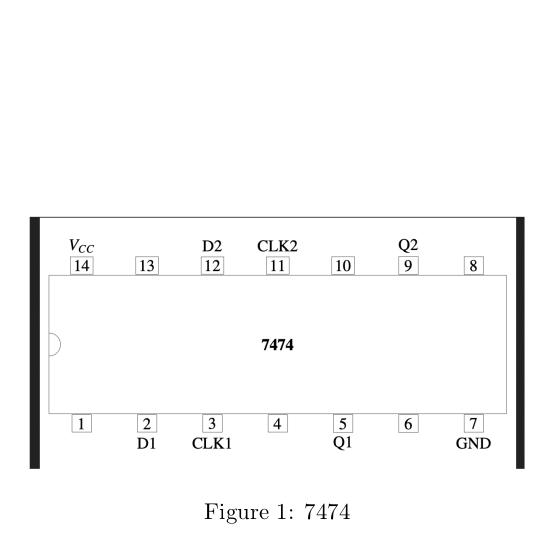
\includegraphics[width=3in]{IC.png}
	\caption{7474}
	\label{fig:circuit}	
\end{figure}
\begin{figure}
	\centering
	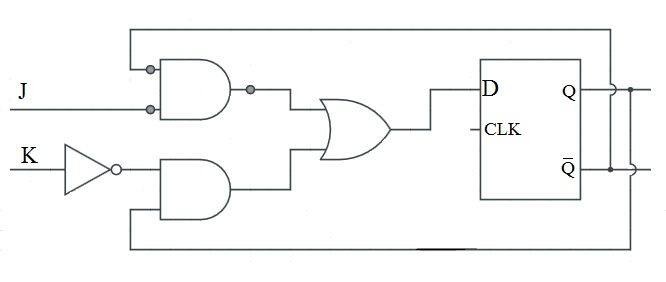
\includegraphics[width=3in]{flip.jpg}
	\caption{Circuit Diagram}

\end{figure}
 \begin{karnaugh-map}[4][2][1][$KQ$][$J$]
        \minterms{1,5,4,6}
        \maxterms{0,2,3,7}
        \indeterminants{2,5}
        \implicant{4}{4}{green}
        \implicant{6}{6}{green}
        \implicant{1}{5}
    \end{karnaugh-map}
%\documentclass[tikz, border=2mm]{standalone}
%\usepackage{karnaugh-map}

\end{document}


